%
% teil1.tex -- Beispiel-File für das Paper
%
% (c) 2020 Prof Dr Andreas Müller, Hochschule Rapperswil
%
\section{Lösung
\label{parzyl:section:teil1}}
\rhead{Lösung}
Zur Lösung der Helmholtz-Gleichung müssen erst die Lösungen der separierten
Differentialgleichungen \eqref{parzyl:sep_dgl_1} bis \eqref{parzyl:sep_dgl_3}
gefunden werden.
\subsection{Lösung der Schwingungsgleichung \eqref{parzyl:sep_dgl_3}}
\eqref{parzyl:sep_dgl_3} beschriebt einen ungedämpften harmonischen Oszillator.
Die Lösung ist somit
\begin{equation}
	i(z) 
	= 
	A\cos{ 
		\left ( z
		\sqrt{\lambda + \mu}
		\right )}
	+
	B\sin{ 
		\left ( z
		\sqrt{\lambda + \mu}
		\right )}.
\end{equation}
\subsection{Lösung der Weberschen Differentialgleichung}
Die Differentialgleichungen \eqref{parzyl:sep_dgl_1} und \eqref{parzyl:sep_dgl_2} werden in \cite{parzyl:whittaker}
mit Hilfe der Whittaker Gleichung gelöst.
\begin{satz}
	Die Funktionen 
	\begin{equation}
		 M_{k,m}(x) = 
		    e^{-x/2} x^{m+1/2} \,
		    {}_{1} F_{1}
		    (
		        {\textstyle \frac{1}{2}} 
		        + m - k, 1 + 2m; x) \qquad x \in \mathbb{C}
		 \label{parzyl:eq:sol_diffEq_1}
	\end{equation}
	und damit auch die Linearkombinationen 
	 \begin{equation}
		        W_{k,m}(x) = \frac{
		            \Gamma \left( -2m\right)
		        }{
		            \Gamma \left( {\textstyle \frac{1}{2}} - m - k\right)
		        }
		        M_{-k, m} \left(x\right)
		        +
		        \frac{
		            \Gamma \left( 2m\right)
		        }{
		            \Gamma \left( {\textstyle \frac{1}{2}} + m - k\right)
		        }
		       M_{k, -m} \left(x\right)
		      \label{parzyl:eq:sol_diffEq_2}
	\end{equation}
	sind Lösungen der Differentialgleichung 
	\begin{equation}
		        \frac{d^2W}{d x^2} +
		        \biggl( -\frac{1}{4}  + \frac{k}{x} + \frac{\frac{1}{4} - m^2}{x^2} \biggr) W = 0.
		        \label{parzyl:eq:whitDiffEq}
	\end{equation}
	
\end{satz}
\begin{definition}
	Die Differentialgleichung \ref{parzyl:eq:whitDiffEq}  heisst Whittaker-Differentialgleichung. Die Funktionen \ref{parzyl:eq:sol_diffEq_1} und \ref{parzyl:eq:sol_diffEq_2} sind Teil der Familie der Whittaker-Funktionen.
\end{definition}
%\begin{definition}
%    Die Funktionen
%    \begin{equation*}
%        M_{k,m}(x) = 
%    e^{-x/2} x^{m+1/2} \,
%    {}_{1} F_{1}
%    (
%        {\textstyle \frac{1}{2}} 
%        + m - k, 1 + 2m; x) \qquad x \in \mathbb{C}
%    \end{equation*}
%    und
%    \begin{equation*}
%        W_{k,m}(x) = \frac{
%            \Gamma \left( -2m\right)
%        }{
%            \Gamma \left( {\textstyle \frac{1}{2}} - m - k\right)
%        }
%        M_{-k, m} \left(x\right)
%        +
%        \frac{
%            \Gamma \left( 2m\right)
%        }{
%            \Gamma \left( {\textstyle \frac{1}{2}} + m - k\right)
%        }
%        M_{k, -m} \left(x\right)
%    \end{equation*}
%    gehören zu den Whittaker Funktionen und sind Lösungen
%    der Whittaker Differentialgleichung
%    \begin{equation}
%        \frac{d^2W}{d x^2} +
%        \biggl( -\frac{1}{4}  + \frac{k}{x} + \frac{\frac{1}{4} - m^2}{x^2} \biggr) W = 0.
%        \label{parzyl:eq:whitDiffEq}
%    \end{equation}
%
%\end{definition}
Es wird nun die Differentialgleichung bestimmt, welche
\begin{equation}
    w = x^{-1/2} W_{k,-1/4} \left({\textstyle \frac{1}{2}} x^2\right)
\end{equation}
als Lösung hat.
Dafür wird $w$ in \eqref{parzyl:eq:whitDiffEq} eingesetzt, woraus
\begin{equation}
    \frac{d^2 w}{dx^2} - \left(\frac{1}{4} x^2 - 2k\right) w = 0
\label{parzyl:eq:weberDiffEq}
\end{equation}
resultiert. Diese Differentialgleichung ist dieselbe wie 
\eqref{parzyl:sep_dgl_1} und \eqref{parzyl:sep_dgl_2}, welche somit
$w$ als Lösung haben.
%Da es sich um eine Differentialgleichung zweiter Ordnung handelt, hat sie nicht nur
%eine sondern zwei Lösungen.
%Die zweite Lösung der Whittaker-Gleichung ist $W_{k,-m} (z)$.
%Somit hat \eqref{parzyl:eq:weberDiffEq}
%\begin{align}
%    w_1(k, z) & = z^{-1/2} W_{k,-1/4} \left({\textstyle \frac{1}{2}} z^2\right)\\
%    w_2(k, z) & = z^{-1/2} W_{k,1/4} \left({\textstyle \frac{1}{2}} z^2\right)
%\end{align}
%als Lösungen.
%Mit der Hypergeometrischen Funktion ausgeschrieben ergeben sich die Lösungen
%\begin{align}
%	\label{parzyl:eq:solution_dgl}
%    w_1(k,z) &= e^{-z^2/4} \,
%    {}_{1} F_{1}
%    (
%        {\textstyle \frac{1}{4}} 
%         - k, {\textstyle \frac{1}{2}} ; {\textstyle \frac{1}{2}}z^2) \\
%    w_2(k,z) & = z e^{-z^2/4} \,
%         {}_{1} F_{1}
%         ({\textstyle \frac{3}{4}} 
%              - k, {\textstyle \frac{3}{2}} ; {\textstyle \frac{1}{2}}z^2).
%\end{align}
\subsection{Standardlösungen}
In der Literatur gibt es verschiedene Standardlösungen für 
\eqref{parzyl:eq:weberDiffEq}, wobei die Differentialgleichung jeweils 
unterschiedlich geschrieben wird.
Whittaker und Watson zeigen in \cite{parzyl:whittaker} die Lösung
\begin{equation}
    D_n(x) = 2^{\frac{1}{2}n + \frac{1}{2}} x^{-\frac{1}{2}} W_{n/2 + 1/4, -1/4}\left(\frac{1}{2}x^2\right),
\end{equation}
welche die Differentialgleichung
\begin{equation}
    \frac{d^2D_n(x)}{dx^2} + \left(n + \frac{1}{2} - \frac{1}{4} x^2\right)D_n(x) = 0
\end{equation}
löst.
Mit $M_{k,m}(x)$ geschrieben resultiert
\begin{equation}
    D_n(x) = \frac{
            \Gamma \left( {\textstyle \frac{1}{2}}\right) 2^{\frac{1}{2}n + \frac{1}{4}} x^{-\frac{1}{2}}
        }{
            \Gamma \left( {\textstyle \frac{1}{2}} - {\textstyle \frac{1}{2}} n \right)
        }
        M_{\frac{1}{2} n + \frac{1}{4}, - \frac{1}{4}} \left(\frac{1}{2}x^2\right)
        +
        \frac{
            \Gamma\left(-{\textstyle \frac{1}{2}}\right) 2^{\frac{1}{2}n + \frac{1}{4}} x^{-\frac{1}{2}}
        }{
            \Gamma\left(- {\textstyle \frac{1}{2}} n\right)
        }
        M_{\frac{1}{2} n + \frac{1}{4}, \frac{1}{4}} \left(\frac{1}{2}x^2\right).
\end{equation}


In \cite{parzyl:abramowitz-stegun} sind zwei Lösungen $U(a, x)$ und $V(a,x)$ 
\begin{align}
    U(a,x) &= 
    \cos\left[\pi \left({\textstyle \frac{1}{4}} + {\textstyle \frac{1}{2}} a\right)\right] Y_1
    - \sin\left[\pi \left({\textstyle \frac{1}{4}} + {\textstyle \frac{1}{2}} a\right)\right] Y_2 
    \label{parzyl:eq:Uaz}
    \\
    V(a,x) &= \frac{1}{\Gamma \left({\textstyle \frac{1}{2} - a}\right)} \left\{
    \sin\left[\pi \left({\textstyle \frac{1}{4}} + {\textstyle \frac{1}{2}} a\right)\right] Y_1
    + \cos\left[\pi \left({\textstyle \frac{1}{4}} + {\textstyle \frac{1}{2}} a\right)\right] Y_2
    \right\}
    \label{parzyl:eq:Vaz}
\end{align}
mit
\begin{align}
    Y_1 &= \frac{1}{\sqrt{\pi}} 
            \frac{\Gamma\left({\textstyle \frac{1}{4} - 
            {\textstyle \frac{1}{2}}a}\right)}
            {2^{\frac{1}{2} a + \frac{1}{4}}}
            e^{-x^2/4} 
            {}_{1} F_{1}
                \left({\textstyle \frac{1}{2}}a + {\textstyle \frac{1}{4}}, 
                {\textstyle \frac{1}{2}} ; 
                {\textstyle \frac{1}{2}}x^2\right)\\
        Y_2 &= \frac{1}{\sqrt{\pi}} 
            \frac{\Gamma\left({\textstyle \frac{3}{4} - 
            {\textstyle \frac{1}{2}}a}\right)}
            {2^{\frac{1}{2} a - \frac{1}{4}}} 
            x e^{-x^2/4} 
            {}_{1} F_{1}
                \left({\textstyle \frac{1}{2}}a + {\textstyle \frac{3}{4}}, 
                {\textstyle \frac{3}{2}} ; 
                {\textstyle \frac{1}{2}}x^2\right)
\end{align}
der Differentialgleichung
\begin{equation}
    \frac{d^2 y}{d x^2} - \left(\frac{1}{4} x^2 + a\right) y = 0
\end{equation}
beschrieben. Die Lösungen $U(a,z)$ und $V(a, z)$ können auch durch $D_n(z)$
ausgedrückt werden
\begin{align}
    U(a,x) &= D_{-a-1/2}(x) \\
    V(a,x) &= \frac{\Gamma \left({\textstyle \frac{1}{2}} + a\right)}{\pi}
    \left[\sin\left(\pi a\right) D_{-a-1/2}(x) + D_{-a-1/2}(-x)\right].
\end{align}
In den Abbildungen \ref{parzyl:fig:dnz} und \ref{parzyl:fig:Vnz} sind 
die Funktionen $D_n(x)$ und $V(a,x)$ mit verschiedenen Werten für $a$ abgebildet.
\begin{figure}
    \centering
    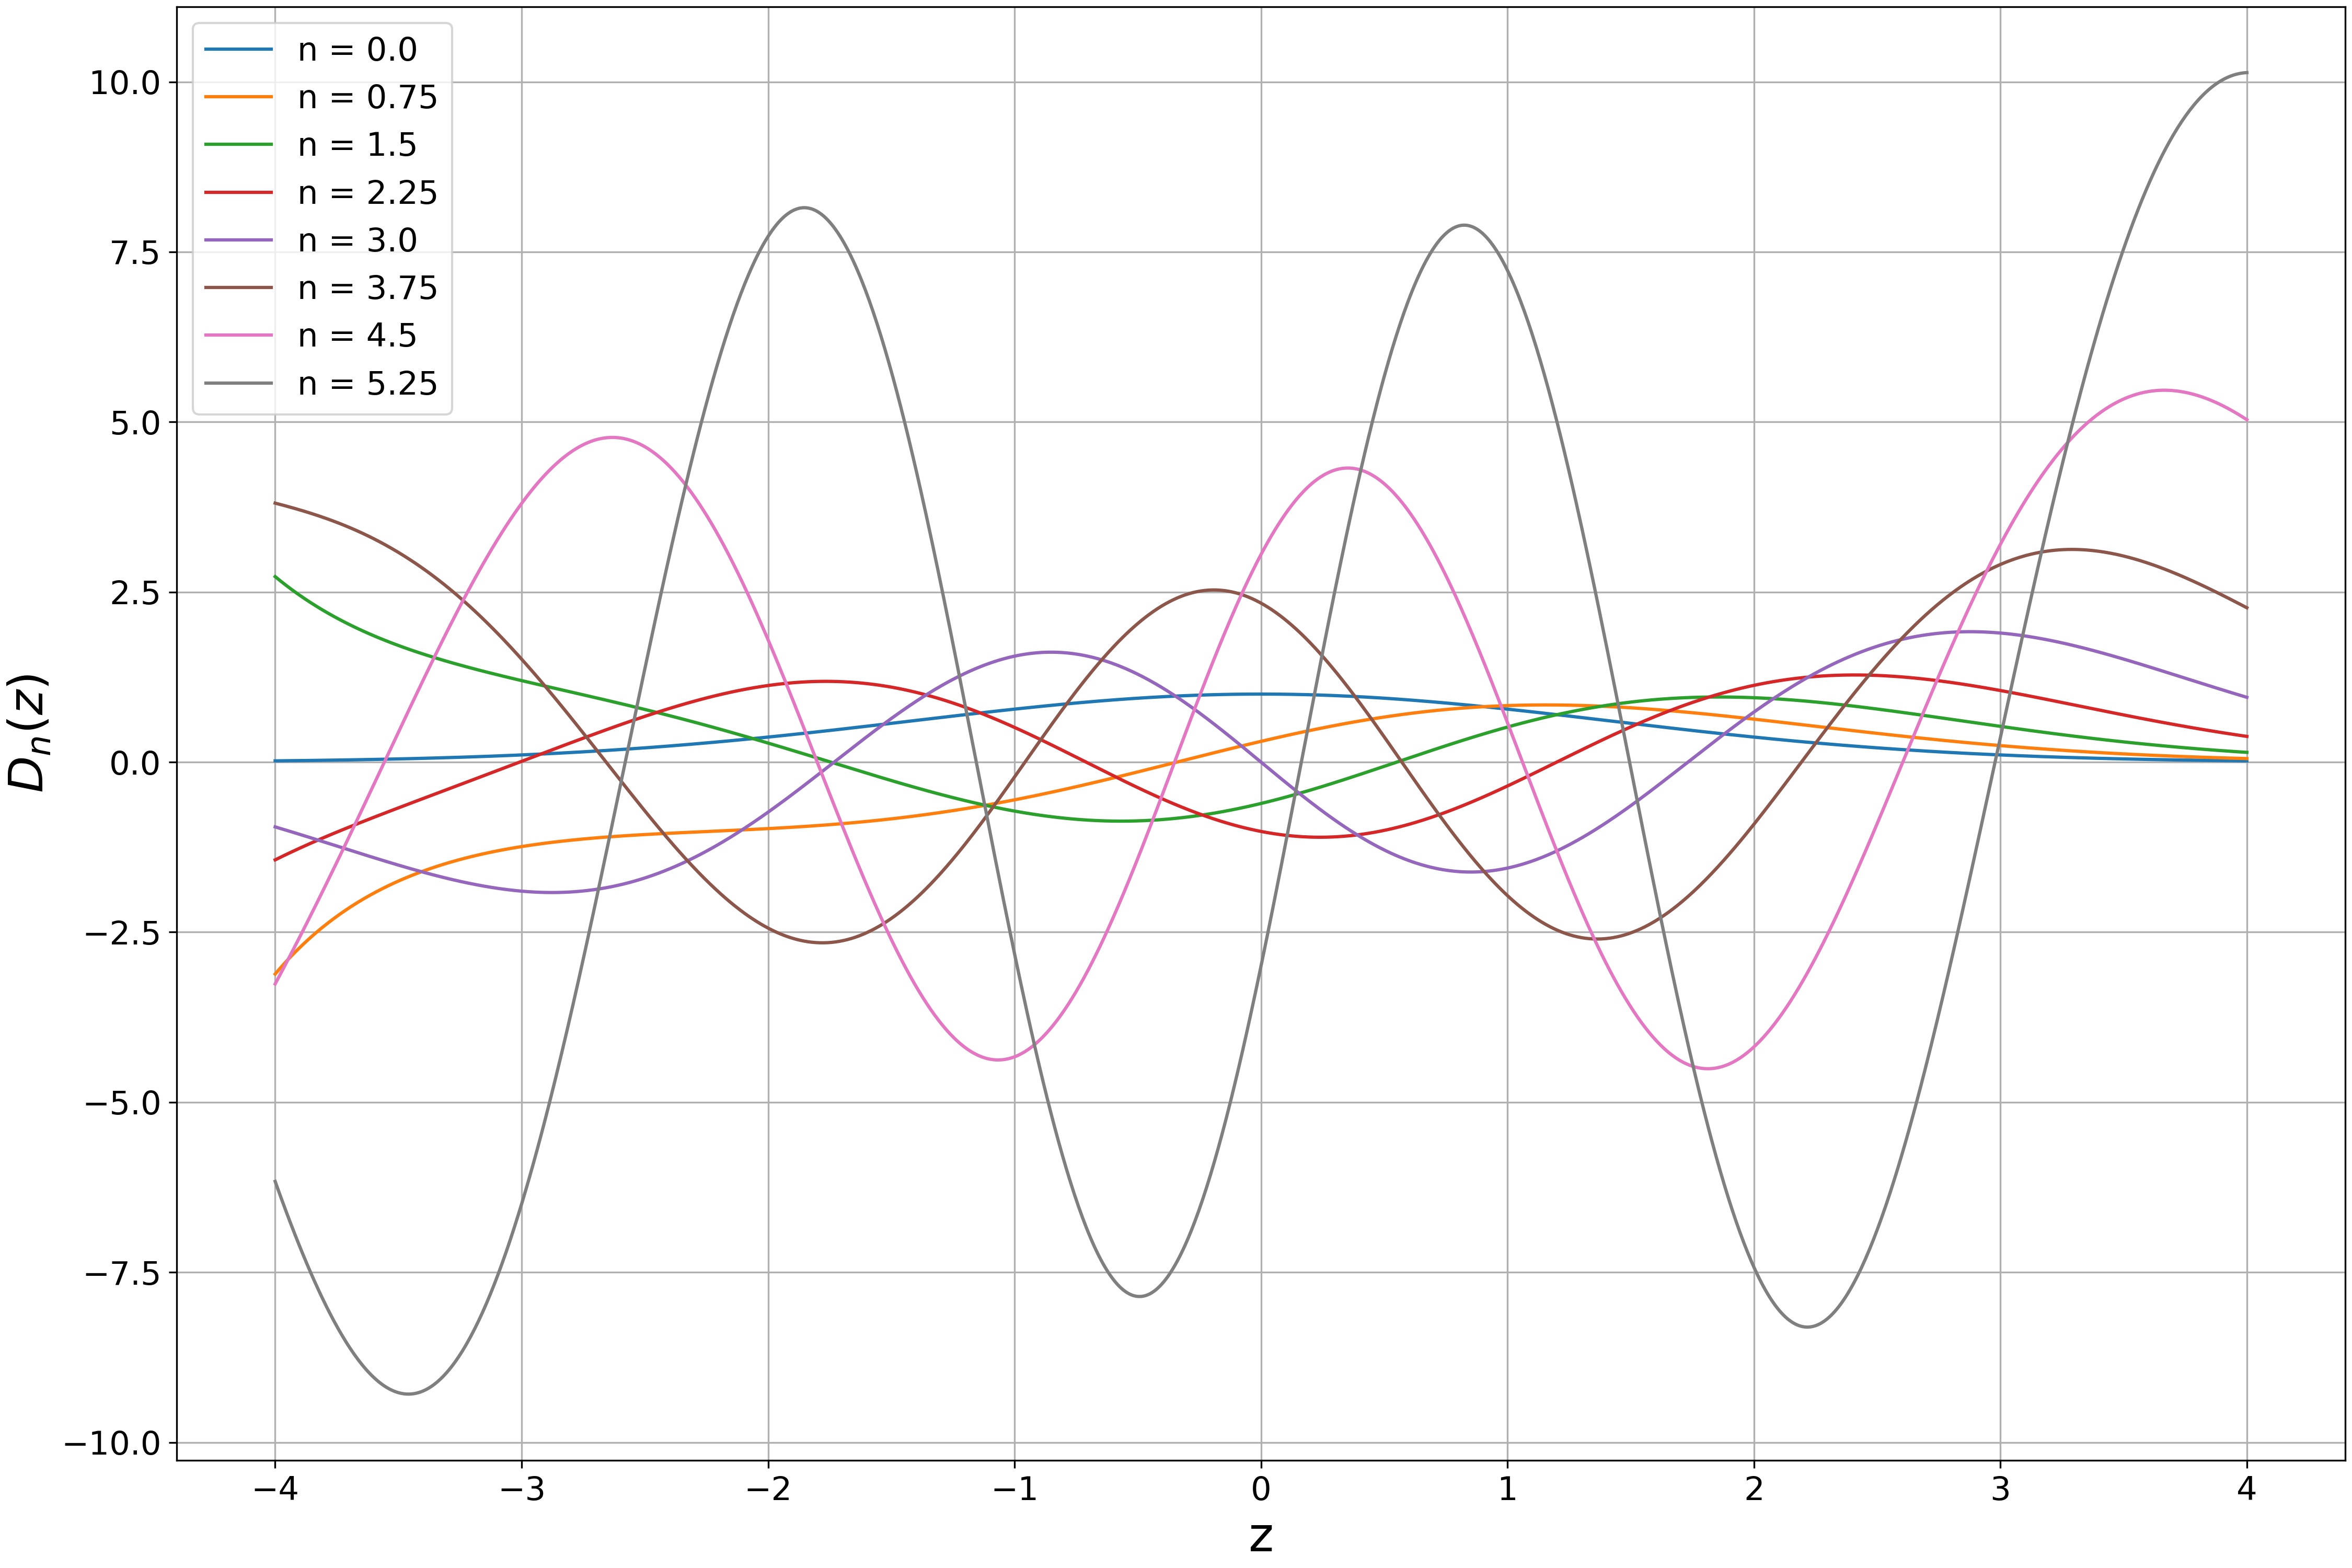
\includegraphics[scale=0.35]{papers/parzyl/img/D_plot.png}
    \caption{$D_n(x)$ mit unterschiedlichen Werten für $n$.}
    \label{parzyl:fig:dnz}
\end{figure}
\begin{figure}
    \centering
    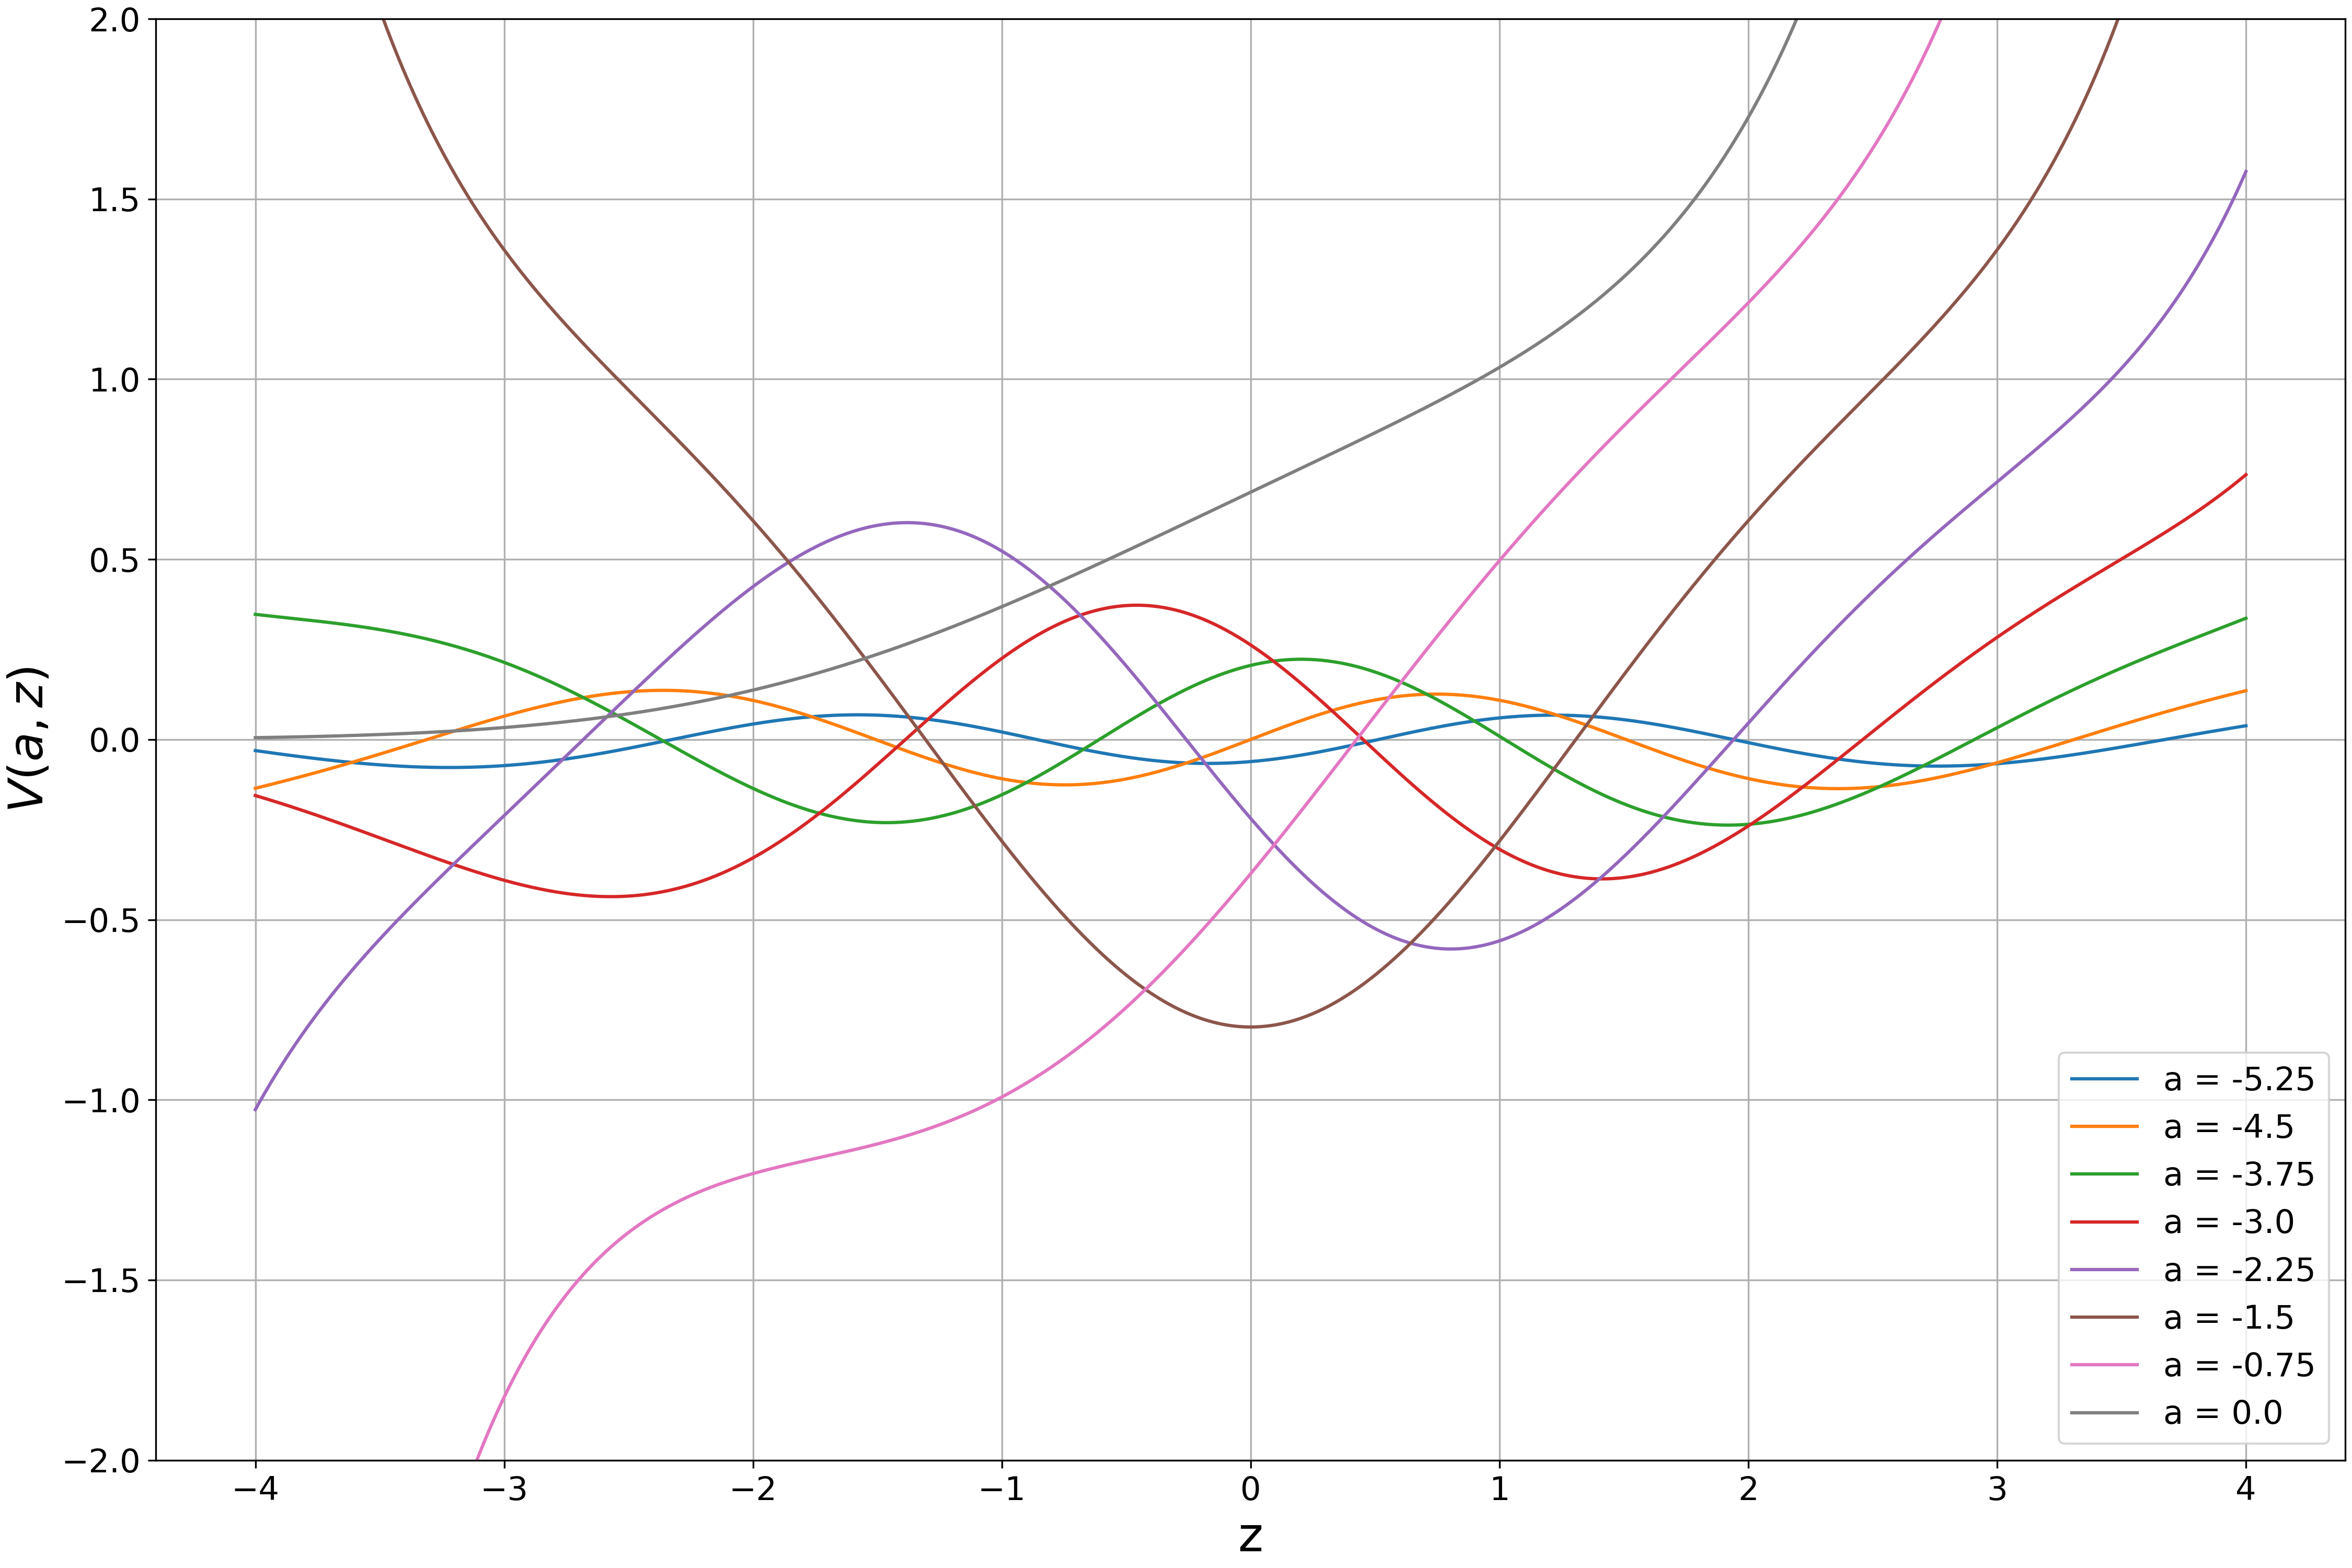
\includegraphics[scale=0.35]{papers/parzyl/img/v_plot.png}
    \caption{$V(a,x)$ mit unterschiedlichen Werten für $a$.}
    \label{parzyl:fig:Vnz}
\end{figure}